\subsection{Constraints on possible pointing strategies}
\label{sec:constraints_on_pointings}
The main constraint on \tesss spatial orientation is that its cameras must oppose the sun.
Specifically, the camera center must point within $\sim30^\circ$ of immediately antisolar, with $\lesssim15^\circ$ preferred.
%\todo[inline]{Roland: are these numbers still good? are they imposed by the sunshade? or solar panels? Some comment appreciated.} 
This is necessary for the sunshade and spacecraft to block solar photons.
It also enables the solar panels (which are free to rotate about the $+Y$ axis in Fig.~\ref{fig:spacecraft_angles}) to collect sunlight.
Given the spacecraft's orbit~\citep{gangestad_high_2013}, this means that \tess should advance $\sim28^\circ$ east in ecliptic longitude every lunar month, as it does during the primary mission.
Focusing on a fixed field for say, 3 spacecraft orbits ($\sim42$ days), would be in tension with this requirement.
In practice, another technical restriction is whether the Earth or Moon passes through \tesss camera fields during a proposed pointing (see Sec.~\ref{sec:earth_moon_crossings}).
For purposes of exploring possible science in extended missions, the spacecraft's finite fuel reserves can be ignored.

\begin{figure}[t] %[!thb]
	\centering
	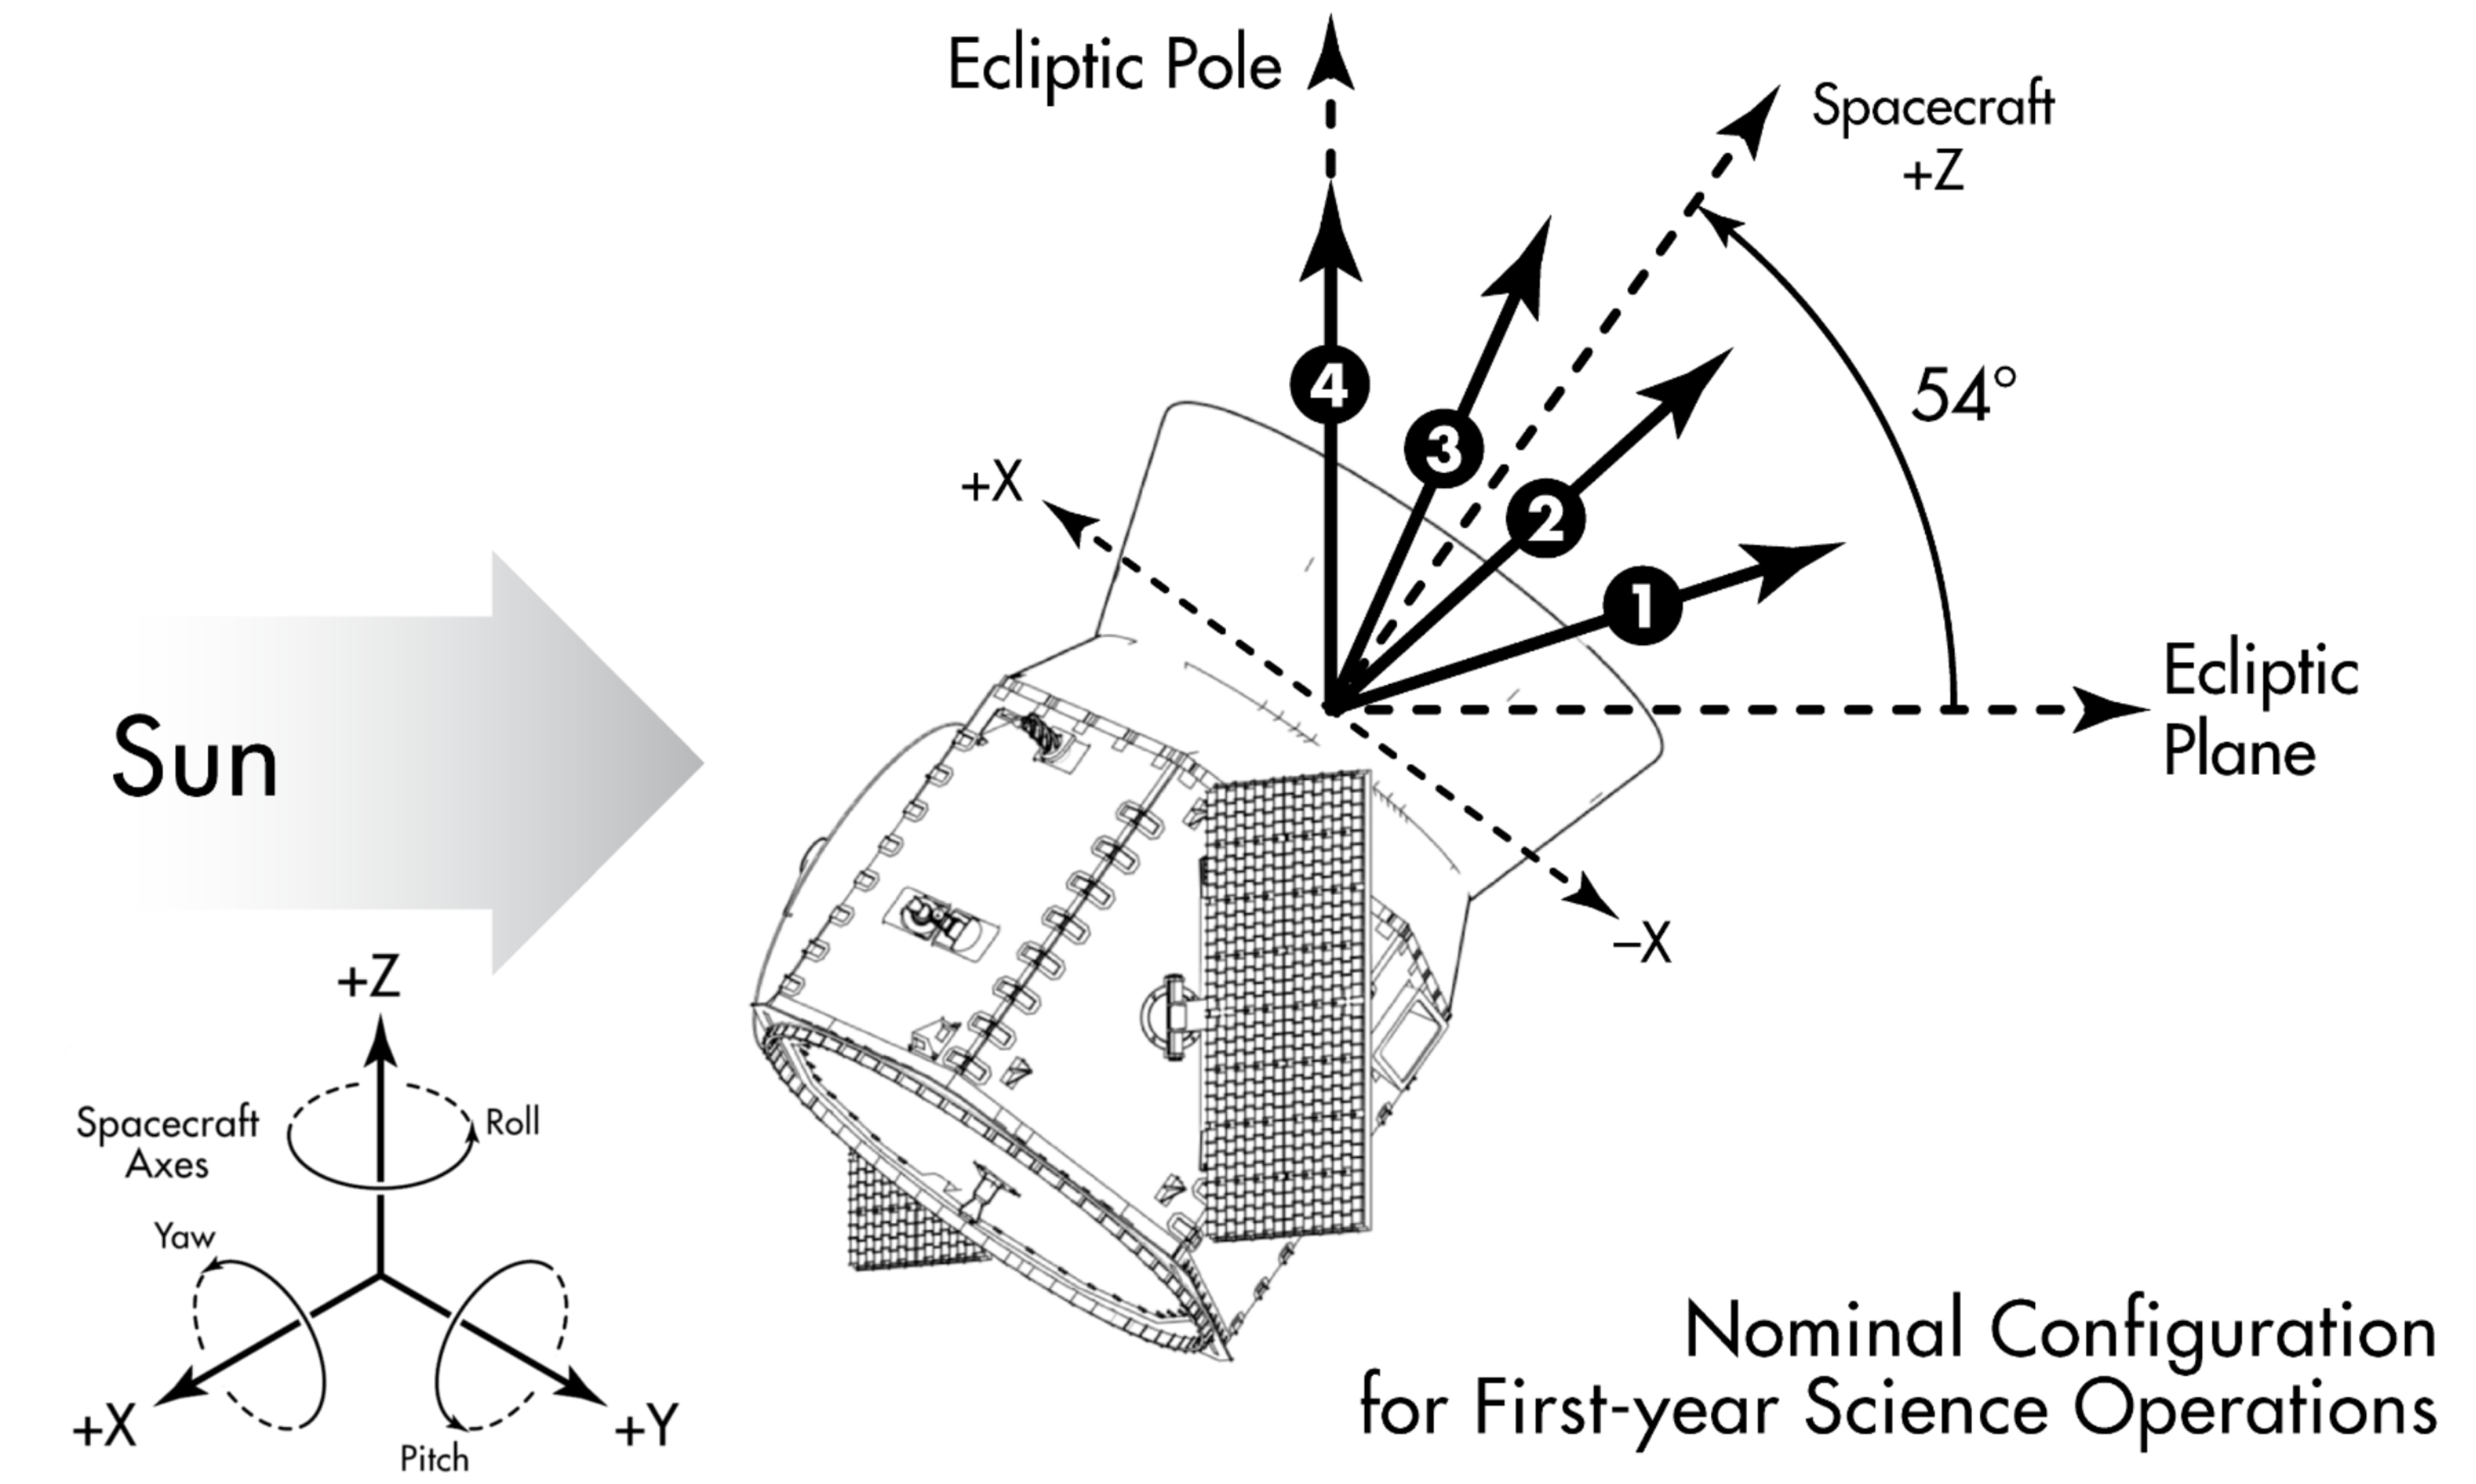
\includegraphics{figures/spacecraft_angles.pdf}
	%\missingfigure{foobar}	
	\caption{\tesss solar panels pitch about the $+Y$ axis. The spacecraft must point so that incident sunlight is collected by the solar panels, and not the cameras. (Adapted from Orbital ATK design document) }
	\label{fig:spacecraft_angles}
\end{figure}